% 3_methodology.tex

\cleardoublepage
\chapter{Launch Vehicle Baseline Design}\label{chapter:methodology}

This chapter presents the design of the baseline launch system, along with aerodynamic and engine performance characteristics. The designs of the three stages of the small satellite launch system are detailed. The launch system has been designed based on the SPARTAN vehicle developed by Preller \& Smart [CITATIONXX], and is shown in Figures \ref{fig:NoInternal} \& \ref{fig:INTERNALS}. The size and external design of the SPARTAN are used exactly as defined for the Baseline SPARTAN vehicle defined by Preller \& Smart, and are not modified in any way. The internal component masses of the SPARTAN are either identical to those defined by Preller \& Smart, or are scaled if the internal component is modified. The first stage rocket, third stage rocket, and internal components have been designed to conform to the size and shape of the Baseline SPARTAN vehicle.
The modified Baseline SPARTAN design is presented first, as the design of the SPARTAN drives the design of the first and third stage rockets. 


\begin{figure}
	\centering
	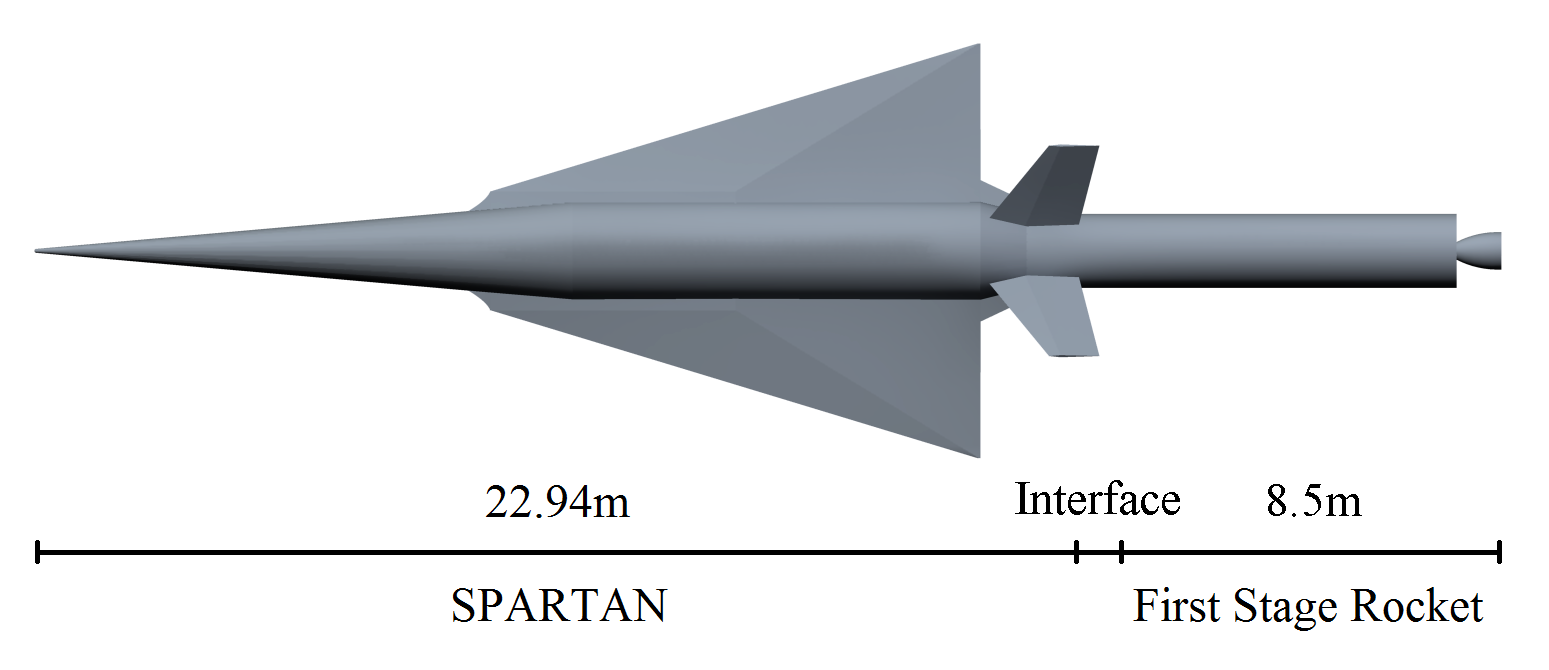
\includegraphics[width=0.7\linewidth]{figures/3_vehicle_design/NoInternal}
	\caption{The rocket-scramjet-rocket launch system, top view, showing the SPARTAN and first stage.}
	\label{fig:NoInternal}
\end{figure}

\begin{figure}
	\centering
	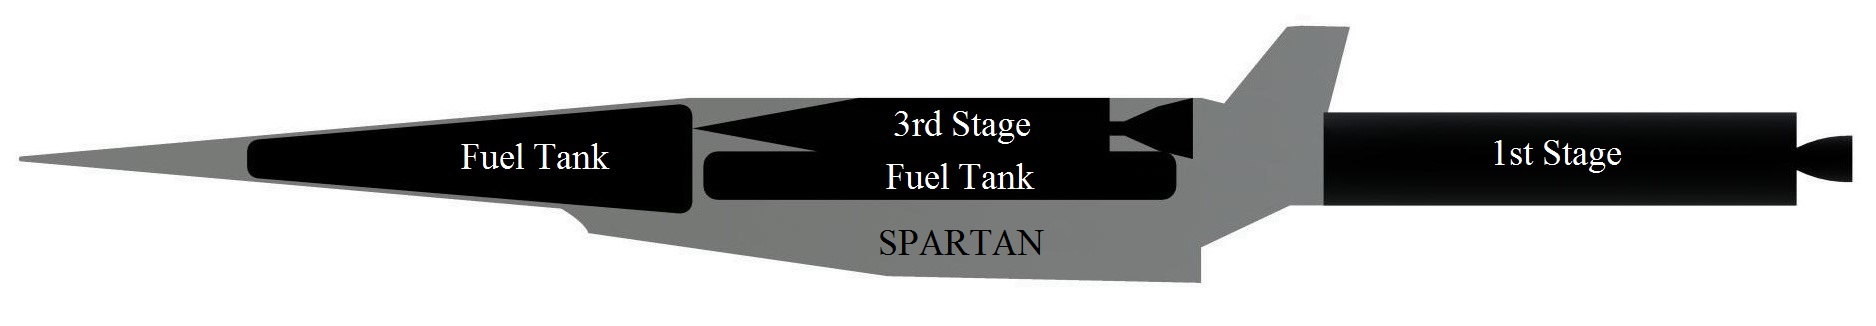
\includegraphics[width=0.7\linewidth]{figures/3_vehicle_design/INTERNALS}
	\caption{The rocket-scramjet-rocket launch system, side view, showing the SPARTAN and fuel tanks, along with the third and first stages.}
	\label{fig:INTERNALS}
\end{figure}





 The trajectory of a launch system involving scramjet propulsion is significantly different to that of a fully rocket-powered launch system, with significant impact on the vehicle design. The operation of the scramjet engine requires in-atmosphere flight at high dynamic pressure conditions. Figure \ref{fig:Trajsimple} shows a simplified representation of the launch trajectory for the vehicle simulated in this study. The launch system is launched vertically under rocket power, from a traditional small rocket launch facility. The SPARTAN vehicle is mounted to the front of the first stage rocket. This configuration allows the SPARTAN to take the brunt of the aerodynamic forces and heating, as well as allowing the use of the control surfaces of the SPARTAN. During first stage rocket operation, the launch system pitches rapidly, reaching close to horizontal flight. The SPARTAN is accelerated to its minimum operating velocity of approximately Mach 5, at which point separation occurs. The SPARTAN's four scramjet engines are ignited, and SPARTAN accelerated through the atmosphere, reaching approximately Mach 9. At this point, the specific impulse of the scramjet engines, and thus the efficiency of the SPARTAN, have decreased, and the third stage rocket is separated. The third stage rocket accelerates and performs a pull-up, before cutting its engine and coasting out of the atmosphere. Once the rocket is exoatmospheric, the engine is reignited multiple times, performing first a circularisation burn, and then a Hohmann transfer to the intended orbit. Meanwhile, the SPARTAN banks and executes a fly-back manoeuvre to return to its initial launch site. The SPARTAN extends landing gear, and lands on a traditional runway in the style of a conventional aircraft. The SPARTAN is able to be rapidly refurbished and remounted for further launches. 


\begin{figure}
	\centering
	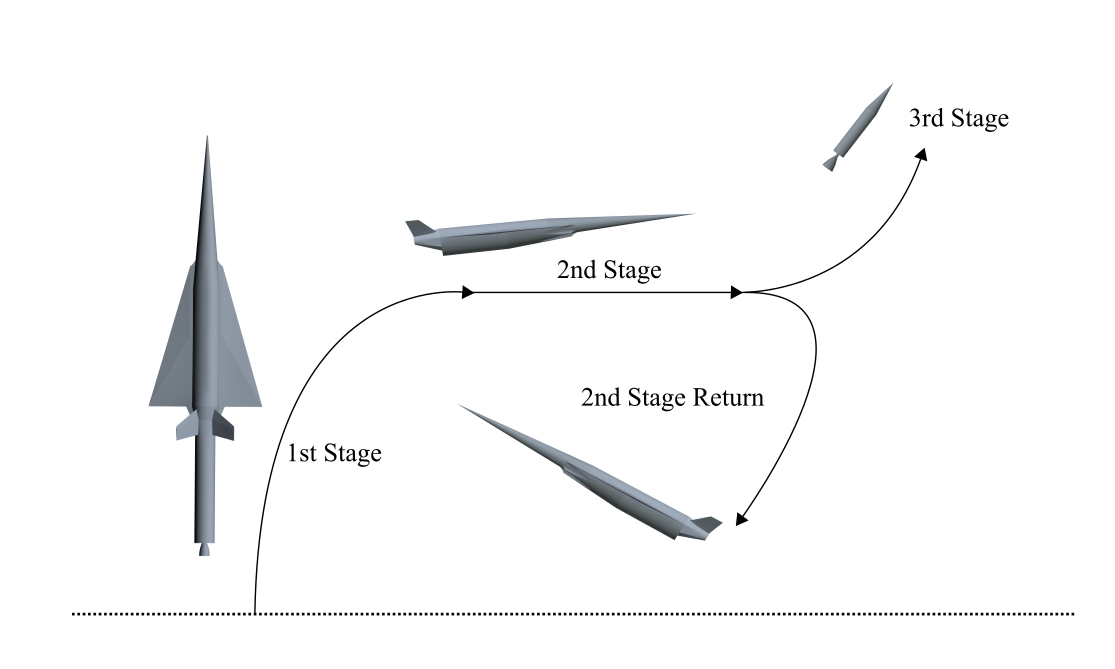
\includegraphics[width=0.9\linewidth]{figures/3_vehicle_design/Trajsimple}
	\caption{The launch process of the rocket-scramjet-rocket launch system, presented in simplified form.}
	\label{fig:Trajsimple}
\end{figure}




	
	
	\section{Second Stage Scramjet}

	
		\subsection{Baseline SPARTAN Vehicle}
		The SPARTAN is a scramjet-powered accelerator being developed by The University of Queensland and Hypersonix. 
		The SPARTAN vehicle in this study has been designed based on the work by Preller \& Smart CITATION. The SPARTAN is 22.94m long, with a frontal cone half angle of 5$^\circ$ [CITEXX DAWIDS THESIS]. A mass breakdown of the SPARTAN is shown in Table \ref{tab:MassBreakdown}, adapted from [CITAXX Dawids thesis], including the modifications made in this thesis, to the fuel tanks and amount of fuel carried.
		
		\begin{table}[h]
		\begin{tabular}{|c|c|c|c|c|c|c|c|}
			\hline  \textbf{Part} & Fuselage & Wings & Tanks & Systems & Landing Gear & Scramjets & Fuel \\ 
			\hline \textbf{Mass} (kg) & 2861.6 & 350.7 & 179.4 & 707.5 & 188.9 & 669.0 & 1562.0 \\ 
			\hline 
		\end{tabular} 
		\caption{Mass breakdown of the modified SPARTAN vehicle.}
		\label{tab:MassBreakdown}
		\end{table}
		
		

		The internals of the SPARTAN have been modified to accommodate for the new kestrel-powered third stage, described in Section \ref{sec:ThirdStageBaseline}. This study assumes that the third stage is stored within the fuselage of the SPARTAN for simplicity. It is assumed that the release mechanism for the third stage is able to be situated within the available space surrounding the third stage. 
		
		
		% LH2 density
		 %http://webbook.nist.gov/cgi/fluid.cgi?Action=Load&ID=C1333740&Type=SatT&Digits=5&PLow=.5&PHigh=1.5&PInc=.1&RefState=DEF&TUnit=K&PUnit=atm&DUnit=kg/m3&HUnit=kJ/mol&WUnit=m/s&VisUnit=uPa*s&STUnit=N/m%

		The fuel tanks are sized to fit around the kestrel-powered third stage. There are three fuel tanks; two cylindrical tanks situated underneath the third stage; and a truncated conical tank in the nose. The conical fuel tank is designed to fit immediately forward of the third stage. This fuel tank is 8m long, leaving 1.47m$^3$ of space in the nose for cooling systems, frontal landing gear and any additional systems or sensors which are necessary in the nose cone. The cylindrical tanks are positioned underneath and slightly to either side of the third stage, leaving space underneath for vehicle systems. The cylindrical fuel tanks are designed to be 8.5m long, with diameters of 0.87m, sized to give a nominal total tank volume of 22m$^3$.
The fuel tanks hold a total of 1562kg of LH2 fuel. This assumes an LH2 density of 71kg/m3, slightly denser than LH2 at phase transition point at 1 atm.
The mass of the fuel tanks is scaled from Dawid Preller's Baseline vehicle model of the SPARTAN, giving a total fuel tank mass of 179.4kg.
		

\subsection{Propulsion Modelling}

The flow entering the engine is calculated using the Tayor-Maccoll analysis method for conical shocks[CitationXX]. This calculation is performed in the cone\_shoot program provided for this study by Prof. Michael Smart[CitationXX?]. The flow conditions following the conical shock are shown in Figure \ref{fig:ConicalShock}. 

\begin{figure}
\begin{subfigure}{.5\textwidth}
\centering
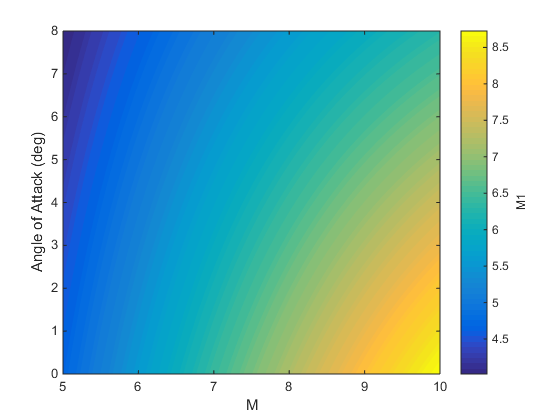
\includegraphics[width=0.99\linewidth]{figures/3_vehicle_design/ConicalM}
\caption{Mach number.}
\label{fig:ConicalM}
\end{subfigure}
\begin{subfigure}{.5\textwidth}
\centering
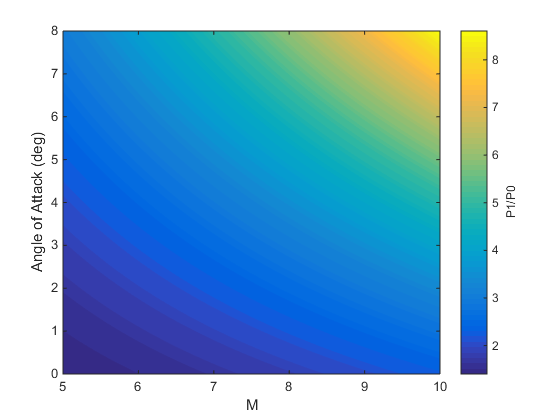
\includegraphics[width=0.99\linewidth]{figures/3_vehicle_design/ConicalP}
\caption{Pressure ratio.}
\label{fig:ConicalP}
\end{subfigure}
\begin{subfigure}{.5\textwidth}
\centering
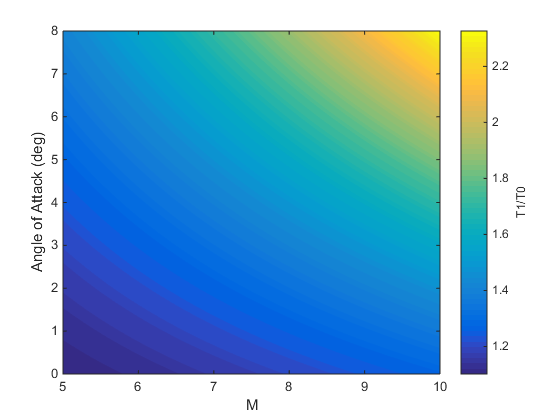
\includegraphics[width=0.99\linewidth]{figures/3_vehicle_design/ConicalT}
\caption{Temperature ratio.}
\label{fig:ConicalT}
\end{subfigure}
\caption{Flow conditions after the conical shock generated by the vehicle nose cone. Figure a) shows the Mach number, b) shows the pressure ratio, and c) shows the temperature ratio following the conical shock.}
\label{fig:ConicalShock}
\end{figure}

The SPARTAN is powered by four underslung scramjet engines. These engines are Rectangular To Elliptical Shape Transition (REST) engines, configured to allow for a conical forebody (C-REST). The engine model used is a CRESTM10 database\cite{Preller2017}, analysed using quasi-1D simulation and provided for this study by Prof. Michael Smart.
This database provides data points of engine performance over inlet conditions within the operational range, at 50kPa dynamic pressure equivalent conditions. The specific impulse data set is shown in Figure \ref{fig:ISPinterp}. This data is interpolated using bivariate splines for the given inlet conditions, to calculate specific impulse produced by the engine. 
For operation at high Mach numbers, the fuel mass flow rate is assumed to be stoichiometric, so that $\dot{m_f}$ = $0.0291\dot{m}$.
\begin{figure}[ht]
	\centering
	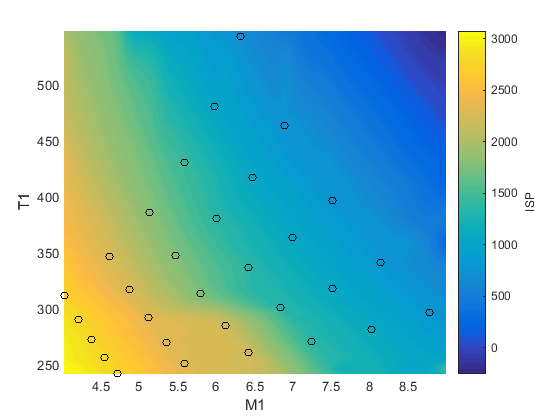
\includegraphics[width=0.6\linewidth]{figures/3_vehicle_design/ISPinterp}
	\caption{Specific impulse of the CRESTM10 engines with input temperature and Mach number. Available data points are indicated.}
	\label{fig:ISPinterp}
\end{figure}
However, the C-REST engine is a fixed geometry engine, primarily designed for operability at high Mach numbers\cite{Preller2017}. At lower Mach numbers, the addition of excessive fuel may cause the engine to choke and unstart, resulting in total loss of thrust\cite{Preller2017}. To avoid unstart, an equivalence ratio ($\phi$) of less than 1 is set at low Mach numbers. As the equivalence ratio is equal to 1 in the majority of the Mach number and temperature regime, only the regions in which it is less than 1 are used for the interpolation. The equivalence ratio interpolation is linear, as the number of data points available for interpolation is low. The equivalence ratio over the range of SPARTAN operation is shown in Figure \ref{fig:EquivalenceRatioInterp}.
\begin{figure}[ht]
	\centering
	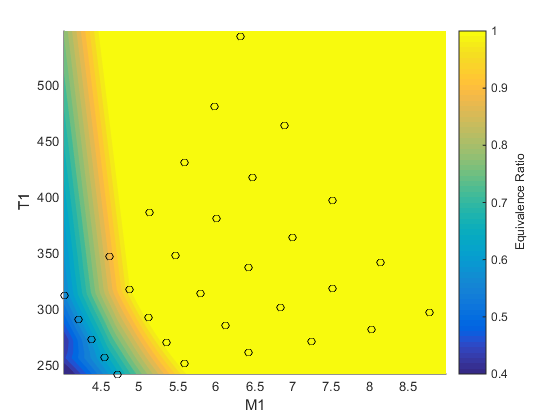
\includegraphics[width=0.6\linewidth]{figures/3_vehicle_design/EquivalenceRatioInterp}
	\caption{Operable equivalence ratio of the CRESTM10 engines with input temperature and Mach number. Available data points are indicated.}
	\label{fig:EquivalenceRatioInterp}
\end{figure}
The mass flow rate is determined by approximating the in flow as an ideal gas; 

$\dot{m}_{fuel} = 0.9 (\dfrac{m_{fuel}}{m_{ox}} )_{st} \phi m_c A_{cap} P_0 M_0 \sqrt{\dfrac{\gamma_0}{R_{air} T_0}}$

\textcolor{red}{Explain details of C-REST calculator here, including mass capture rate and capture area modifiers. Citation for this?}

The multiplier of 0.9 is an approximate term included to account for losses due to asymmetry within the engine. 
The thrust, $T$, is obtained by inclusion of the mass flow rate ($\dot{m}$) obtained via the inlet conditions, ie. $T = g_0\dot{m}I_{sp}$. 

During flight the C-REST inlet conditions will stay within the region bounded by the available data. However, for the purposes of the pseudospectral method solver, it is necessary for the vehicle model to be able to extrapolate for ISP and equivalence ratio data. This extrapolation is linear, and is used to drive the optimisation, but does not directly affect the final solution. 





		
		
		\subsection{Aerodynamics}
		
		The aerodynamics of the SPARTAN have been calculated using CART3D, an inviscid CFD package used in the preliminary design of aerospace vehicles. Cart3D utilises adjoint mesh adaption with a Cartesian cut-cells approach to produce an iteratively refined mesh to fit a flow solution. CART3D has
		been used to generate the aerodynamic database of the SPARTAN vehicle due to its applicability in both the subsonic
		and supersonic regimes, and its robustness across multiple flow solutions [16]. CART3D has previously been used to
		analyse hypersonic vehicles, and has shown fair agreement with experimental data across multiple studies CITATIONXX.
		
		The aerodynamics of the SPARTAN are calculated for engine-on and engine-off conditions, and are trimmed using control surfaces on the wings at every condition. The centre of gravity varies during flight due to fuel consumption and third stage release. Consequently, aerodynamic databases are created for centre of gravity conditions of; 
		\begin{itemize}
			\item full fuel including third stage,
			\item empty of fuel including third stage,
			\item empty of fuel after third stage release.
		\end{itemize}
		At each of these conditions, aerodynamic coefficients and necessary flap deflections are calculated. 
		The process for generating the aerodynamic databases is shown in Figure \ref{fig:FlowChart}. 
		Figure \ref{fig:aero1} shows the engine off aerodynamic characteristics of the SPARTAN vehicle over the range of Mach numbers and angle of attack values analysed.
		
			\begin{figure}
				\centering
				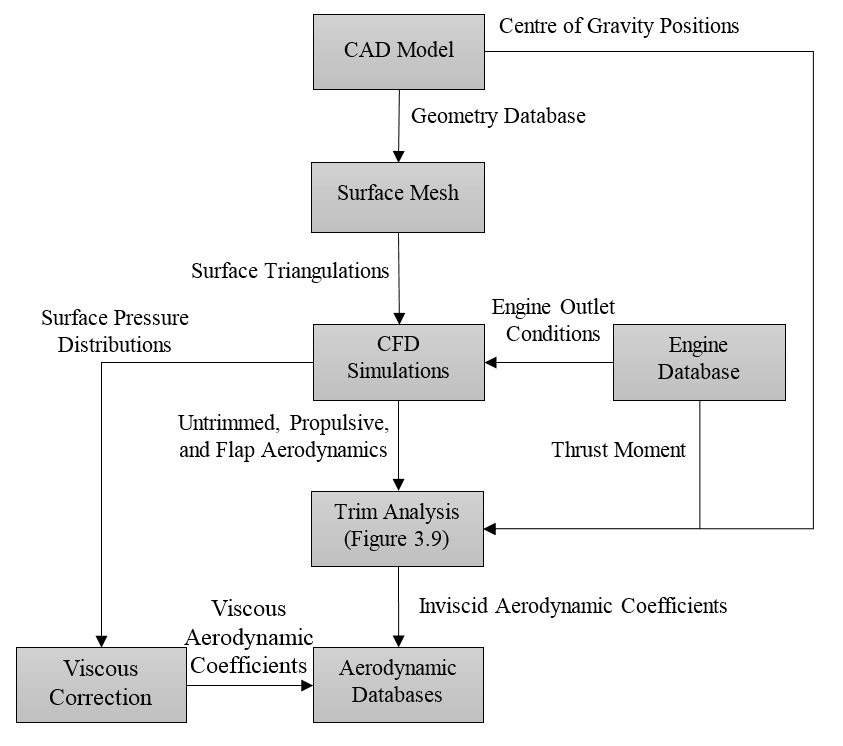
\includegraphics[width=0.7\linewidth]{figures/3_vehicle_design/FlowChart}
				\caption{Process for generating aerodynamic databases.}
				\label{fig:FlowChart}
			\end{figure}
		
		
		
		\subsubsection{CART3D Set-Up}
		
		An initial surface triangulation of the SPARTAN has been created in Pointwise, shown in Figure \ref{fig:Pointwise}. This was imported into CART3D as a watertight surface. 
		CART3D Meshes were initiated with an outer boundary distance of 40 times the vehicle length. This boundary distance was observed to produce suitable free stream conditions and good mesh convergence. Nine mesh adaption levels were used. Nine levels were observed to generally produce good convergence, with moderate computation times of 1-3 hours per simulation. The convergence of the residuals and forces were investigated to ascertain if a solution has converged. Figure XX shows an example solution validation for Mach 7, 2 degrees angle of attack, engine-on. Good convergence can be observed in the force functionals, with a corresponding decrease in the residual values indicating solution convergence.  
		
		
		\textcolor{red}{CART3D validation image here, showing decreasing residuals and converging functionals.}
		
		
		
	
		
		
		
		\begin{figure}[ht]
			\centering
			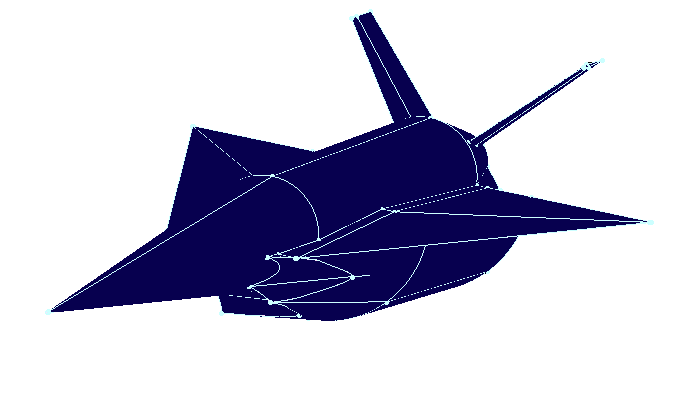
\includegraphics[width=0.6\linewidth]{figures/3_vehicle_design/Pointwise}
			\caption{Surface triangulation of the Baseline SPARTAN.}
			\label{fig:Pointwise}
		\end{figure}
		
		\subsubsection{Engine-Off Aerodynamics}
		
		During the majority of the return flight, the scramjet engines are not operational, and air flows through the flowpath without fuel injection. When the engines are not powered on, the flowpath generates a large amount of drag. 
		The aerodynamics of the SPARTAN are calculated using for Mach numbers from 0.2 to 10, and angle of attack values from 0$^\circ$ to 10$^\circ$. Engine-on aerodynamic calculations are performed for Mach numbers 5,7,9 and 10, and at altitudes from 20km to 40km. An example CART3D solution are shown for a Mach 7 engine off condition is shown in Figure  \ref{fig:M7AoA6}. 
		
		
		\begin{figure}
			\centering
			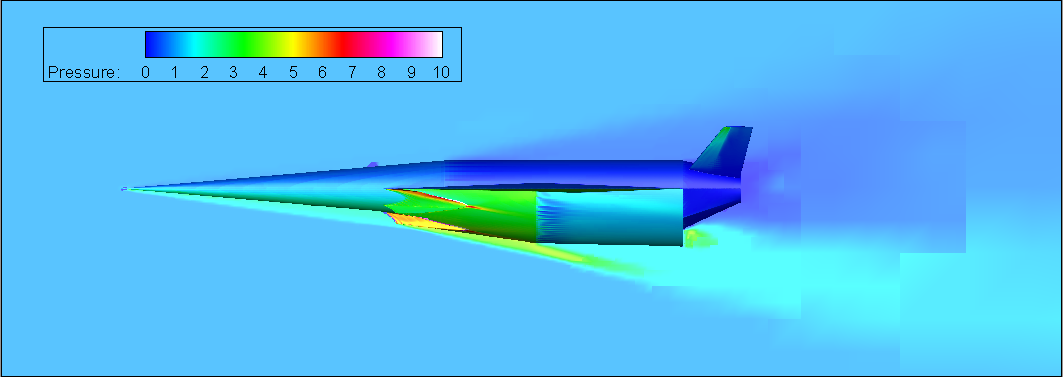
\includegraphics[width=0.9\linewidth]{figures/3_vehicle_design/M7AoA6}
			\caption{CART3D flow result for the SPARTAN, at Mach 7, 6$^\circ$ angle of attack.}
			\label{fig:M7AoA6}
		\end{figure}
		
		\begin{figure}
			\begin{subfigure}{.5\textwidth}
				\centering
				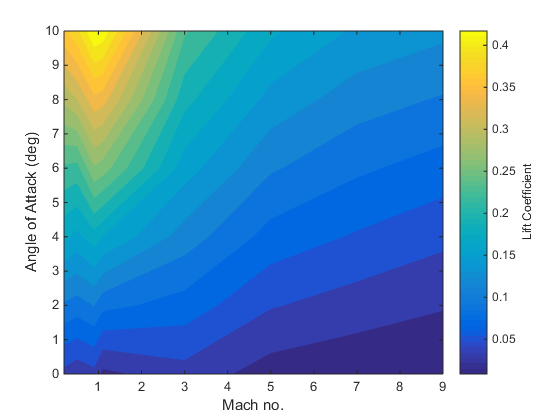
\includegraphics[width=0.99\linewidth]{figures/3_vehicle_design/Cl}
				\caption{Coefficients of lift of the SPARTAN, calculated using CART3D.}
				\label{fig:Cl}
			\end{subfigure}
			\begin{subfigure}{.5\textwidth}
				\centering
				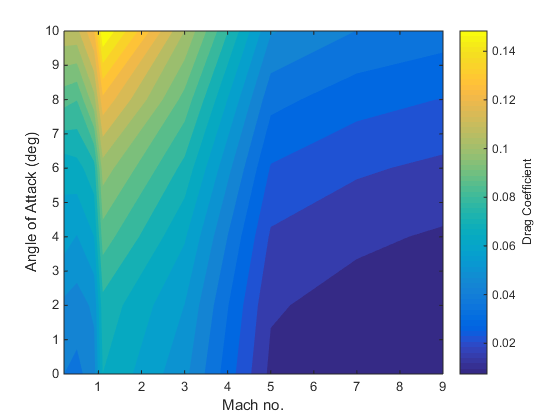
\includegraphics[width=0.99\linewidth]{figures/3_vehicle_design/Cd}
				\caption{Coefficients of drag of the SPARTAN, calculated using CART3D.}
				\label{fig:Cd}
			\end{subfigure}
			\begin{subfigure}{.5\textwidth}
				\centering
				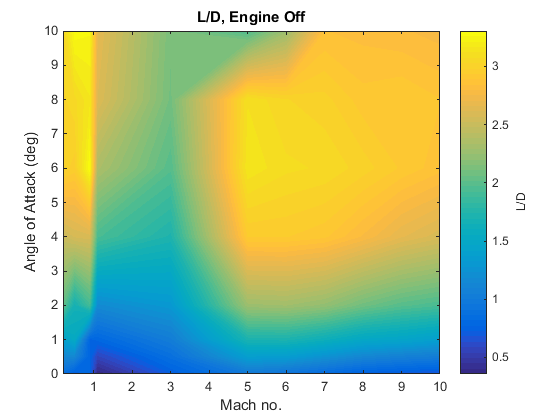
\includegraphics[width=0.99\linewidth]{figures/3_vehicle_design/LD}
				\caption{L/D of the SPARTAN.}
				\label{fig:LD}
			\end{subfigure}
			\caption{Aerodynamic Characteristics of the SPARTAN with C-REST engine off.}
			\label{fig:aero1}
		\end{figure}
		
		These results show a distinct maximum region in the L/D of the SPARTAN at high Mach numbers, within the hypersonic regime. Below Mach 5, the L/D of the SPARTAN decreases sharply. 
		
		
		
		\subsubsection{Engine-On Aerodynamics}\label{sec:engine-on}
		
		The operation of the scramjet engines changes the aerodynamic characteristics of the SPARTAN significantly. When the engines are powered on, the engines are generating thrust on the internal nozzle, as well as on the boat-tail and base. 
		The plumes of the scramjet engines exit the nozzle of the SPARTAN, and are further expanded onto the boat tail on the rear of the SPARTAN fuselage. This expansion causes significant force on the boat tail of the SPARTAN, generating additional lift, thrust and moment forces. The plumes of the SPARTAN have been simulated using CART3D, using SurfBC boundary conditions which produce inflow and outflow conditions at the inlet and exit of the scramjet engines\cite{Pandya2004}. 
		
		\begin{figure}
			\centering
			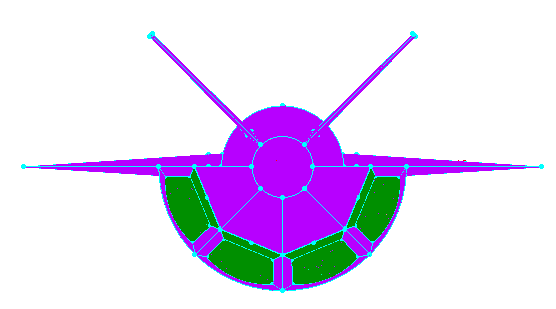
\includegraphics[width=0.7\linewidth]{figures/3_vehicle_design/Pointwise-EngineBC}
			\caption{Pointwise view of the SPARTAN showing engine outlet boundaries.}
			\label{fig:Pointwise-EngineBC}
		\end{figure}
		
		The CRESTM10 database has been used to calculate the engine conditions at the exit of the scramjet engines, and this has been set as the outflow condition. These conditions are normalised for CART3D as follows CITATIONXX:
		
		\begin{equation}
		P_e^* = P_e/(\gamma_0 P_0)
		\end{equation}
		
		\begin{equation}
		\rho_e^* = \rho_e/\rho_0
		\end{equation}
		
		\begin{equation}
		M_e^* = \sqrt{\gamma_e/\gamma_0 (M_e \sqrt{ P_e^*/\rho_e^*})^2}
		\end{equation}
		This includes a correction on the Mach number to account for $\gamma_e$ variation, which is not possible to include directly in CART3D\cite{Mehta2016}.
		
		\begin{figure}
			\centering
			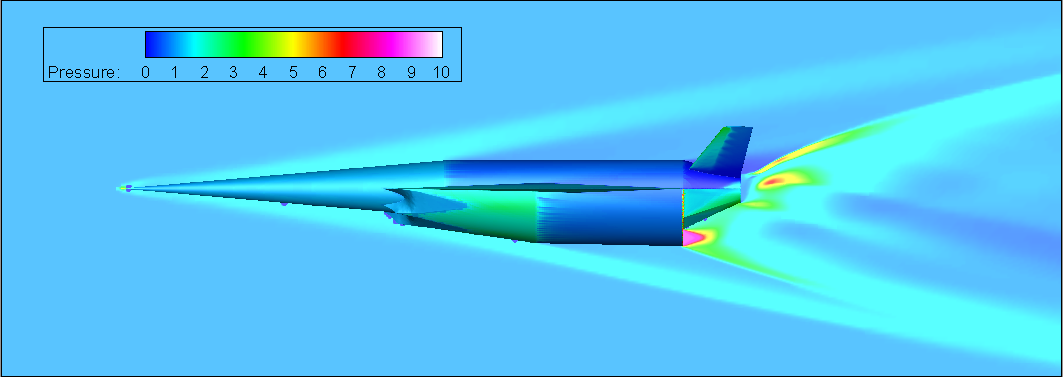
\includegraphics[width=0.9\linewidth]{figures/3_vehicle_design/EngineOn-M7AoA024km}
			\caption{}
			\label{fig:EngineOn-M7AoA624km}
		\end{figure}
		
		
		\begin{figure}
			\begin{subfigure}{.5\textwidth}
				\centering
				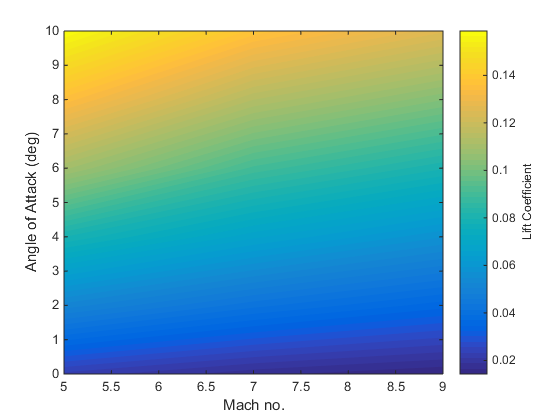
\includegraphics[width=0.99\linewidth]{figures/3_vehicle_design/Cl-EngineOn}
				\caption{Coefficient of lift.}
				\label{fig:Cl-EngineOn}
			\end{subfigure}
			\begin{subfigure}{.5\textwidth}
				\centering
				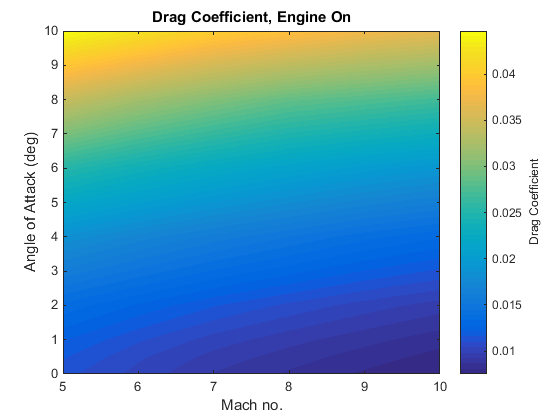
\includegraphics[width=0.99\linewidth]{figures/3_vehicle_design/Cd-EngineOn}
				\caption{Coefficient of drag.}
				\label{fig:Cd-EngineOn}
			\end{subfigure}
			\begin{subfigure}{.5\textwidth}
				\centering
				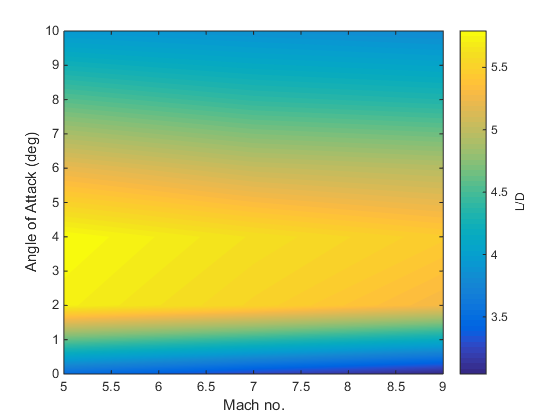
\includegraphics[width=0.99\linewidth]{figures/3_vehicle_design/LD-EngineOn}
				\caption{L/D.}
				\label{fig:LD-EngineOn}
			\end{subfigure}
			\caption{Aerodynamic coefficients with the C-REST engines powered on.}
		\end{figure}
		

		\subsubsection{Trim Analysis}
The centre of gravity of the SPARTAN has been calculated using CREO, based on the mass breakdown in (CITEXX Dawids Thesis). For simplicity, it is assumed that structural, systems and landing gear masses are homogeneously distributed throughout the centre fuselage of the SPARTAN. The calculated centre of gravity for the SPARTAN without the third stage rocket is 14.52m along the body length. 
The centre of gravity of the SPARTAN is varied as fuel is depleted throughout the acceleration phase, as well as when the third stage rocket is released. A point mass model is used in conjunction with the aerodynamic database,
and atmospheric properties obtained from the U.S Standard Atmosphere 1976[26]. The SPARTAN is assumed to be
trimmed at all conditions during flight.
\begin{figure}
	\centering
	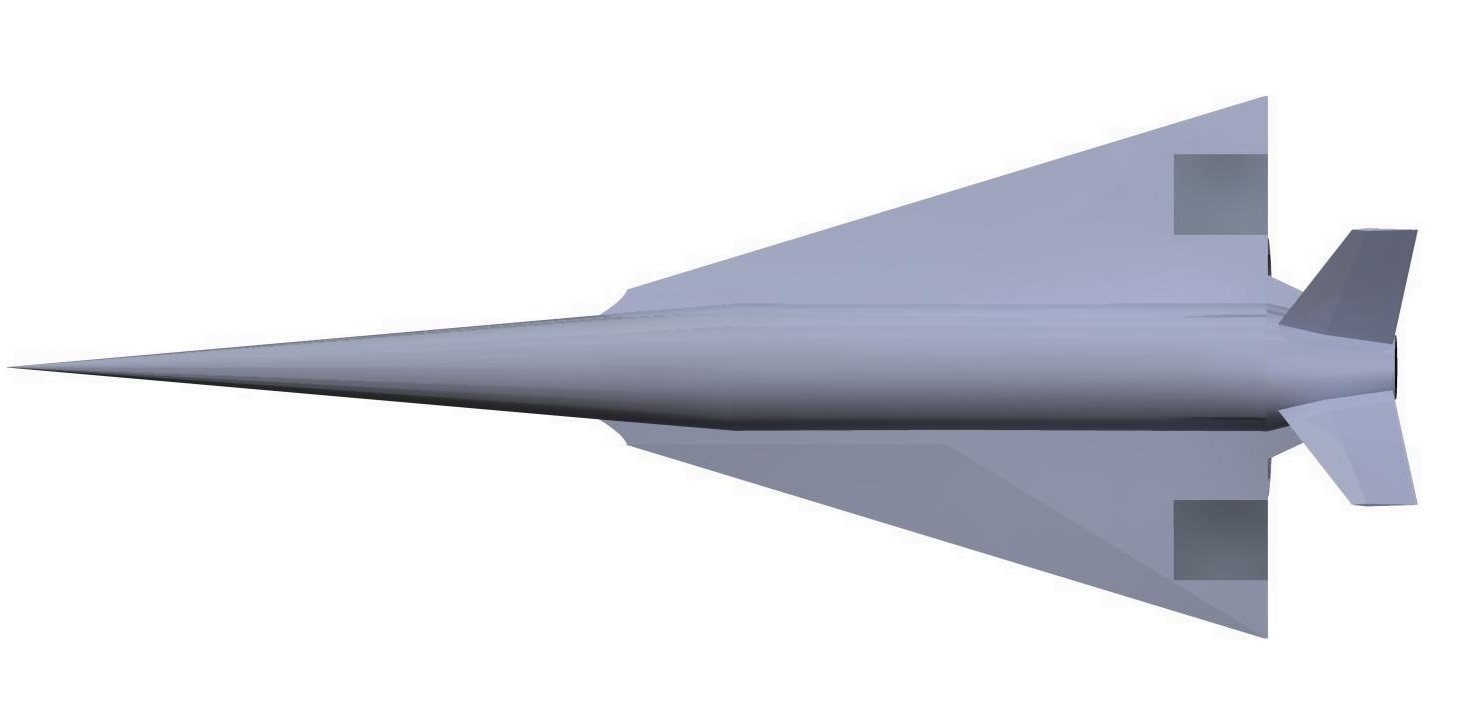
\includegraphics[width=0.7\linewidth]{figures/3_vehicle_design/SPARTAN_FLAPS}
	\caption{}
	\label{fig:SPARTAN_FLAPS}
\end{figure}
The SPARTAN is trimmed using control surfaces on the wings, shown in figure \ref{fig:SPARTAN_FLAPS}. 
The trimmed aerodynamics of the SPARTAN are determined by modelling the flaps at deflected states of -20$^\circ$, -10$^\circ$, 10$^\circ$, and 20$^\circ$. Each of these deflected states were modelled in CREO and a surface mesh was created in Pointwise. The aerodynamics at each flap deflection were calculated at 0$^\circ$ angle of attack for Mach numbers between 0.2 and 10. Trim is determined by calculating the aerodynamic moment coefficient with zero flap deflection, then calculating the flap deflection necessary to balance the aerodynamic moments to zero. This trim balancing is calculated prior to trajectory optimisation for computational efficiency. For each aerodynamic data point of Mach numbers between 0.2 and 10, and angle of attacks from 0$^\circ$ to 10$^\circ$, the necessary flap deflection are calculated, and the additional lift and drag produced by the flaps are added. The addition of trimmed aerodynamics is calculated for scramjet engines on, and engines off conditions. Due to centre of gravity variation, the trim analysis is calculated three times; at the beginning of SPARTAN acceleration; at the end of SPARTAN acceleration, when fuel has been depleted; and after the third stage has been released. The trimmed aerodynamic databases at the beginning and end of acceleration are interpolated between as the centre of gravity varies due to fuel depletion. After the third stage is released, the centre of gravity is kept constant, and a single trimmed aerodynamic database is used. 

Figure \ref{fig:FlapDeflection} shows the necessary flap deflections to trim the SPARTAN. An Engine-on case is shown at a centre of gravity of  XXm corresponding to full-fuel with third stage, and an Engine-off case is shown for a centre of gravity of XXm, corresponding to a fuel-empty state after third stage release. Additional figures illustrating the variation in moment coefficients are shown in Appendix XX.
The flap deflections are designated as negative up. Negative flap deflection necessary for trim indicates that the centre of pressure is aft of the centre of gravity, and that the vehicle has positive static margin, and is generally likely to be stable. Figure \ref{fig:FlapDeflectionENgineOn} and XX indicate that the SPARTAN is stable for 

\begin{figure}
\begin{subfigure}{.5\textwidth}
\centering
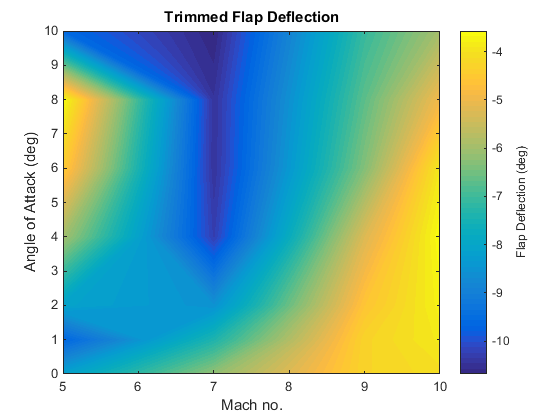
\includegraphics[width=0.99\linewidth]{figures/3_vehicle_design/FlapDeflectionENgineOn}
\caption{}
\label{fig:FlapDeflectionENgineOn}
\end{subfigure}
\begin{subfigure}{.5\textwidth}
	\centering
	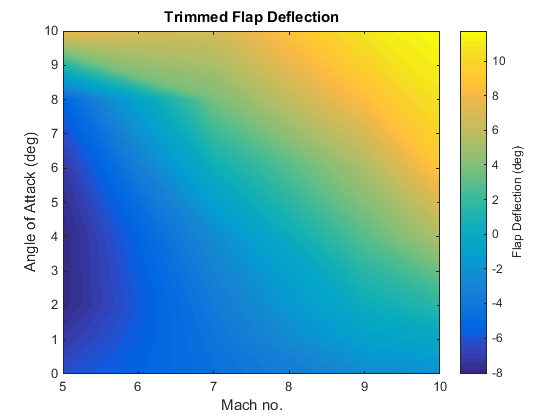
\includegraphics[width=0.99\linewidth]{figures/3_vehicle_design/FlapDeflectionENgineOn2}
	\caption{}
	\label{fig:FlapDeflectionENgineOn2}
\end{subfigure}
\begin{subfigure}{.5\textwidth}
	\centering
	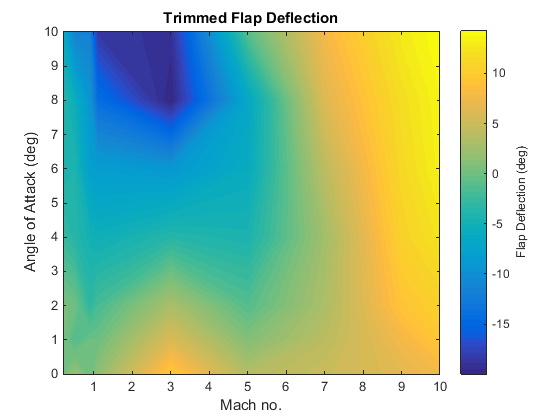
\includegraphics[width=0.99\linewidth]{figures/3_vehicle_design/FlapDeflection}
	\caption{}
	\label{fig:FlapDeflectionEngineOff}
\end{subfigure}
\label{fig:FlapDeflection}
\caption{Flap deflection required for trim of the SPARTAN. Negative up.}
\end{figure}


\section{First Stage Rocket}
The first stage rocket is required to deliver the second stage to near horizontal flight at Mach 5.1 flight conditions,
after which it is discarded. To achieve this, the first stage rocket is modelled as a Falcon-1e first stage scaled down
lengthwise to 9.5m, keeping the original diameter of 1.67m[8]. 
The Falcon-1e has been chosen due to its appropriate scale, and the proven flightworthiness of the Falcon-1. 
 The first stage is attached to the rear of the scramjet
second stage and is powered by a single LOX-kerosene Merlin 1-C engine. This first stage has a structural mass of
1356kg, determined by scaling of the structural mass of the Falcon-1e. The engine mass of the Merlin 1-C is kept constant during scaling at 630kg[CITATIONXX]. The mass of the
fuel in the first stage is scaled as part of the optimisation routine, as the dynamics of the vehicle, and its ability to reach a
given separation point, are very closely coupled to the available fuel mass.

The thrust and specific impulse of the Merlin 1-C are determined by interpolation between the sea level and vacuum specific impulse of the Merlin 1-C, shown in Table XX, with pressure. Thrust scaling is determined by linear pressure scaling using nozzle exit area, $T = T_{SL} + (p_e - p_{SL})A_e$. 
 The Merlin 1-C is throttled down to a constant 85\% to allow the first stage to pitch over more easily.

\begin{tabular}{|c|c|}
	\hline  $I_{SP_{SL}}$ & 275s \\ 
	\hline  $I_{SP_{vac}}$ & 304s\\ 
	\hline  $T_{SL}$ & 555.9kN \\ 
	\hline  $A_{e}$ & $0.552m^2$ \\ 
	\hline 
\end{tabular} 

  \subsubsection{Aerodynamics Including First Stage}

  
  The aerodynamics of the SPARTAN and first stage rocket have been calculated using CART3D. For the purposes of these simulations, a connecting cowl has been modelled between the first stage rocket and the SPARTAN to improve the aerodynamic profile. The first stage aerodynamics have been modelled between angles of attack of 0$^\circ$ to -5$^\circ$, as the first stage will be flying at negative angle of attack to induce faster pitch-over. Mach numbers from 0.2 to 5.1 (second stage separation velocity) have been simulated. Figure \ref{fig:CARTcontour} shows an example CART3D simulation case, at Mach 2, -1$^\circ$ angle of attack. Figure \ref{fig:FirstStageAero} shows the lift and drag coefficients of the first stage, as well as the lift-over-drag, across the simulated Mach Numbers and angles of attack. 
  
  
  
  \begin{figure}
  	\centering
  	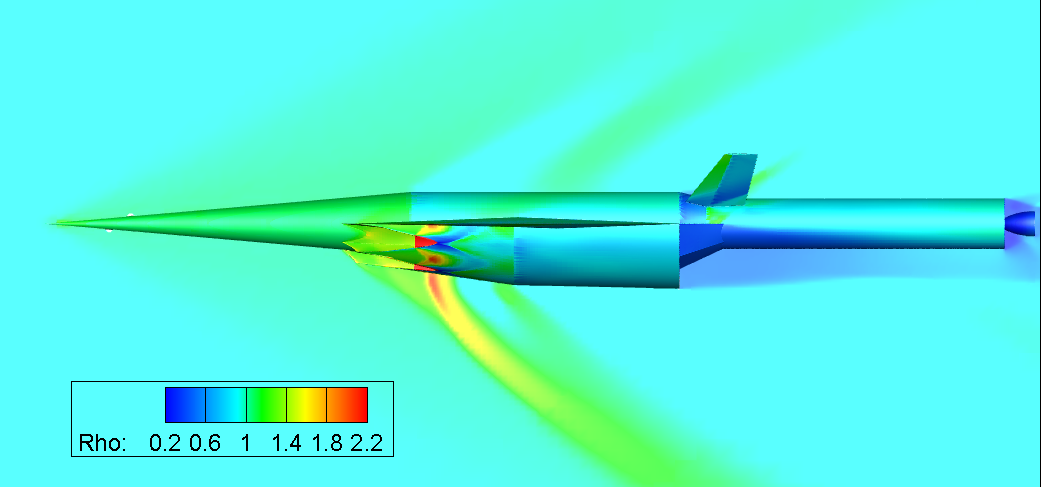
\includegraphics[width=0.7\linewidth]{figures/3_vehicle_design/CARTcontour}
  	\caption{CART3D result for the SPARTAN and first stage vehicles at Mach 2, -1$^\circ$ angle of attack.}
  	\label{fig:CARTcontour}
  \end{figure}

\begin{figure}
	\begin{subfigure}{.5\textwidth}
		\centering
		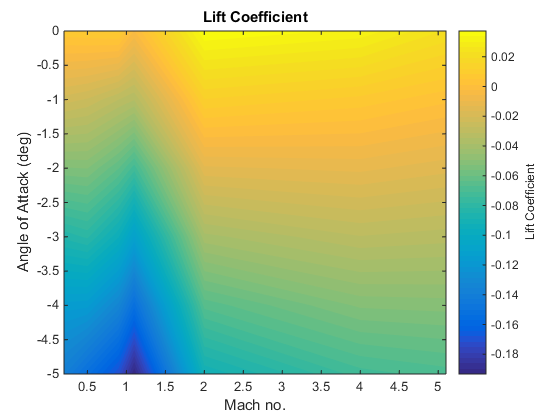
\includegraphics[width=0.99\linewidth]{figures/3_vehicle_design/FirstStageCl}
		\caption{Coefficient of lift.}
		\label{fig:Cl-FirstStage}
	\end{subfigure}
	\begin{subfigure}{.5\textwidth}
		\centering
		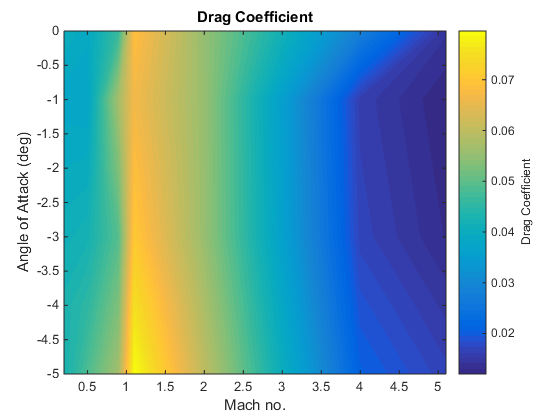
\includegraphics[width=0.99\linewidth]{figures/3_vehicle_design/FirstStageCd}
		\caption{Coefficient of drag.}
		\label{fig:Cd-FirstStage}
	\end{subfigure}
	\begin{subfigure}{.5\textwidth}
		\centering
		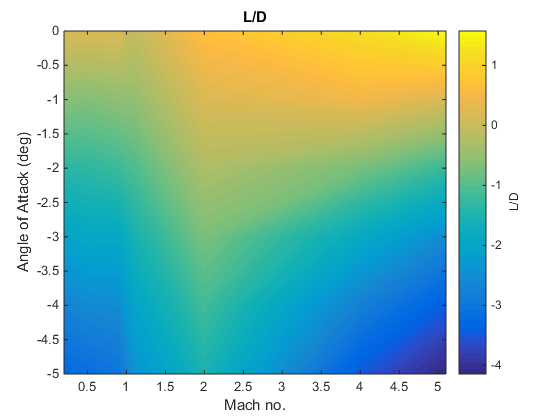
\includegraphics[width=0.99\linewidth]{figures/3_vehicle_design/FirstStageLD}
		\caption{L/D.}
		\label{fig:LD-EFirstStage}
	\end{subfigure}
	\caption{Aerodynamic characteristics of the SPARTAN including the first stage rocket.}
	\label{fig:FirstStageAero}
\end{figure}


	

	\section{Third Stage Rocket - Baseline}\label{sec:ThirdStageBaseline}
	
	\begin{figure}
\centering
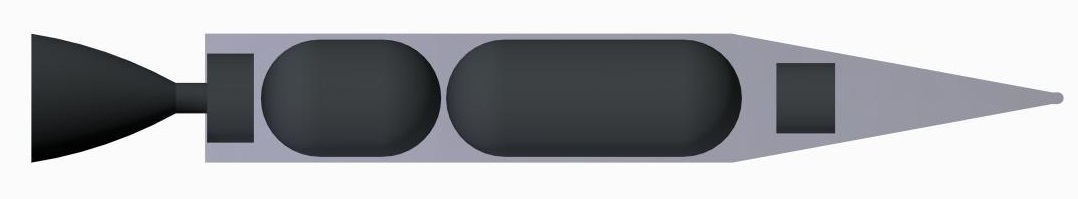
\includegraphics[width=0.7\linewidth]{figures/3_vehicle_design/3rdStage}
\caption{}
\label{fig:3rdStage}
\end{figure}
	
	In this study the third stage rocket has been designed to accommodate a SpaceX Kestrel engine. In previous studies, the third stage was designed to be powered by a Pratt \& Whitney RL-10-3A pump-fed engine, weighing 52kg. The Kestrel has been used over the RL-10-3A for its cost effectiveness. As a pressure-fed engine, the Kestrel trades off specific impulse for weight and cost savings when compared to the RL-10-3A. As the only expendable portion of the system; the cost of the third stage is one of the main drivers of overall system cost. Reducing the cost of the third stage allows the cost of launch to be directly reduced. 
	
	The third stage rocket is released at the end of the scramjet accelerator burn, and lifts the payload out of the atmosphere and into the desired orbit. The third stage weighs a total of 3300kg. This was chosen as a design weight, to fit the fuel necessary to achieve orbit with an acceptable payload while also allowing for ample payload volume. The third stage has a structural mass fraction of 0.09, similar to the Falcon 1 second stage \cite{Vehicle2008}. This gives a total structural mass of 285.7kg. 
	
	

	
The kestrel engine has been modified to have 50\% increased propellant mass flow rate, giving a mass flow rate of 14.8kg/s. The nozzle exit of the Kestrel engine has been kept constant at 1.1m diameter. An increase in mass flow necessitates a corresponding increase in throat area. This increase in throat area decreases the area ratio of the nozzle. The initial area ratio is 60, measured from schematics in the Falcon-1 Users Guide. A 50\% mass flow increase corresponds to a 50\% throat area increase, which causes the area ratio to decrease to 40. This decrease in area ratio results in a 2\% loss of efficiency from the nozzle\cite{RPE}, due to the thrust coefficient decreasing as shown in Figure \ref{fig:ThrustCoefficient-Arat}. The modified specific impulse of the engine is 310.7s.



The third stage has a total length of 9m, with a 3m long nose, 4.5m long centrebody and 1.5m long engine.
	
	The centre of gravity is determined using CREO, and is at XXm from the nose. It is assumed that the mass of the structure of the rocket (excluding fuel tanks, heat shielding, engine and payload) is distributed homogeneously for simplicity.
	
	
	\begin{figure}
\centering
\includegraphics[width=0.7\linewidth]{"figures/3_vehicle_design/Thrust Coefficient - Arat"}
\caption{\cite{RPE}}
\label{fig:ThrustCoefficient-Arat}
\end{figure}



\subsection{Heat Shield Sizing}
\textcolor{red}{present more of the logic which led to this heat shield design}

The third stage rocket is separated from the SPARTAN at a high dynamic pressure, after which it spends a considerable amount of time accelerating in-atmosphere before reaching exoatmospheric conditions. This release into a high dynamic pressure environment creates a large amount of heating, which must be mitigated by heat shielding. 
The third stage is protected while in-atmosphere by a heat shield, weighing 125.6kg. This heat shield is constructed from a phenolic cork cylinder, a reinforced carbon-carbon nose cone, and a tungsten nose tip. 


\begin{tabular}{|c|c|c|c|}
	\hline  Part & Density & Geometry & mass \\ 
	\hline  Tungsten Nose & $\rho_{Tungsten} = 19.25$  g/cm$^3$ & 50mm diameter cylinder, spherical tip & 12.6kg \\ 
		\hline C-C Cone & $\rho_{CC} = 1800$  kg/m$^3$ & 10mm thick, conical & 89.3kg \\ 
			\hline Phenolic Cork Cylinder & $\rho_{Phenolic Cork} = 320$  kg/m$^3$ & 5mm thick, cylindrical & 23.7kg \\ 
	\hline 
\end{tabular} 
		
		\subsection{Fuel Tank Sizing}
		The internal design of the third stage is allowed to be slightly variable as the trajectory is optimised. The third stage mass is fixed at 3300kg, and the calculated payload-to-orbit varies by exchanging leftover fuel mass for effective payload mass. To calculate the dynamics of the third stage, the fuel tanks have been approximately sized, assuming 160kg of payload-to-orbit. Realistically the exchange between fuel and payload mass would cause the fuel tanks to be resized slightly. For the purposes of this study the fuel tanks have been assumed to be of constant size for simplicity. Currently this is a reasonable assumption as the internals of the rocket are very simplified. The structural mass is held constant at 9\%. The third stage carries a total propellant mass of 2736.7kg. Table XX breaks shows the component break-down of the LOX oxidiser and RP1 fuel.  
		
\begin{tabular}{|c|c|c|}
	\hline  & \textbf{LOX} & \textbf{RP1} \\ 
	\hline Ratio & 2.56 & 1 \\ 
	\hline Density & 1141kg/m3 & 813kg/m3 \cite{Magee}\\ 
	\hline Volume & 1.7248m3 & 0.9455m3 \\ 
	\hline Mass & 1968.0 kg & 768.7 kg \\ 
	\hline 
\end{tabular} 
		
		

		\subsection{Aerodynamics}
		
		The third stage aerodynamics have been calculated using Missile DATCOM [REFXX], a preliminary design tool for estimating the aerodynamic characteristics of missile and rocket vehicles. Missile DATCOM utilises empirical methods, along with various estimation techniques, to compute the aerodynamics of missile-like vehicles across the subsonic, supersonic and hypersonic regimes.  The code used to compute the aerodynamics of the third stage rocket is detailed in Appendix XX.  
		
		
		\begin{figure}
			\begin{subfigure}{.5\textwidth}
				\centering
				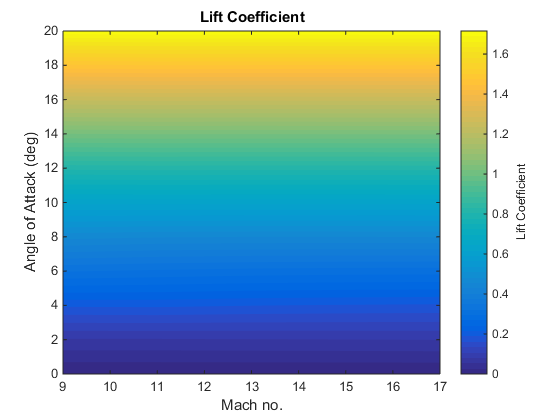
\includegraphics[width=0.99\linewidth]{figures/3_vehicle_design/ThirdStageCl}
				\caption{Coefficient of lift.}
				\label{fig:Cl-ThirdStage}
			\end{subfigure}
			\begin{subfigure}{.5\textwidth}
				\centering
				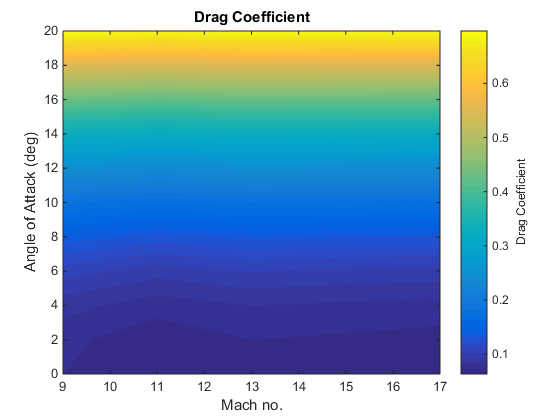
\includegraphics[width=0.99\linewidth]{figures/3_vehicle_design/ThirdStageCd}
				\caption{Coefficient of drag.}
				\label{fig:Cd-ThirdStage}
			\end{subfigure}
			\begin{subfigure}{.5\textwidth}
				\centering
				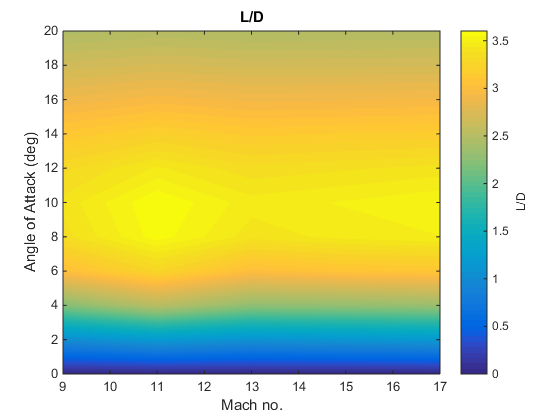
\includegraphics[width=0.99\linewidth]{figures/3_vehicle_design/ThirdStageLD}
				\caption{L/D.}
				\label{fig:LD-ThirdStage}
			\end{subfigure}
			\caption{Aerodynamic characteristics of the baseline third stage rocket, for a reference area of 0.95m$^2$.}
			\label{fig:ThirdStageAero}
		\end{figure}
		
		
		
		\subsection{Thrust Vectoring}
		
		The third stage rocket is trimmed during the in-atmosphere portion of its ascent trajectory via thrust vectoring. The centre of pressure is calculated using missile DATCOM. The thrust vector is set so that the moment generated by the engine matches the lift force acting at the centre of pressure. The maximum thrust vector limit has been set to 8$^\circ$. As no data on the maximum thrust vectoring capabilities of the kestrel engine was able to be found, this was set to the maximum gimbal range of the Aestus pressure-fed engine and OMS, similar pressure fed engines.
		
		The third stage rocket is statically unstable. Flying this rocket at an angle of attack will require an advanced automatic controller, as the only control available is produced by thrust vectoring. This study assumes that the third stage rocket is able to be controlled over any required trajectory, within the thrust vector limits of the vehicle. 
		
		
\begin{figure}
\centering
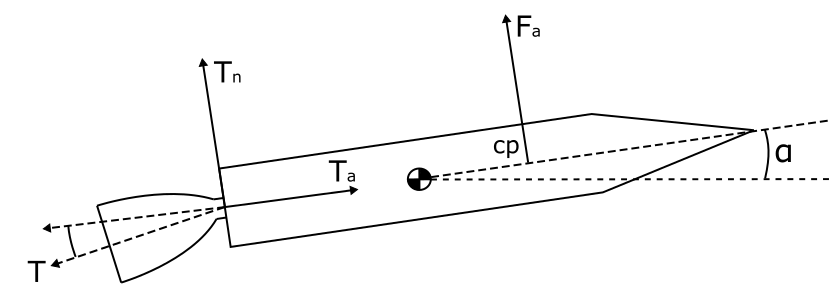
\includegraphics[width=0.6\linewidth]{figures/3_vehicle_design/ThrustVec}
\caption{}
\label{fig:ThrustVec}
\end{figure}
		

		